\section{Análisis multifractal}

\subsection{Relación entre multifractalidad y robustez}

El análisis multifractal provee una herramienta para examinar la estructura de una red. Ahora, se va hacer una relación entre esa medida y algunas redes. Las estrategias de ataque fueron definidas en el capitulo \ref{cap5}.

Las redes de estudio son:

\begin{enumerate}
    \item Red A: Red libre de escala 8000 nodos
    \item Red B: Red de mundo pequeño 5000 nodos, probabilidad de reconexión 10\%
    \item Red C: Red aleatoria 1991 nodos
    \item Red D: Red observada en bacteria C.elegans
    \item Red E: Red fractal (1,3)-flower
\end{enumerate}

Debido a que se debe ejecutar el análisis de multifractalidad a medida que se pierde un porcentaje de nodos, se utiliza el algoritmo SandBox.

\subsubsection{Red libre de escala}

\begin{figure}[H]
    \centering
    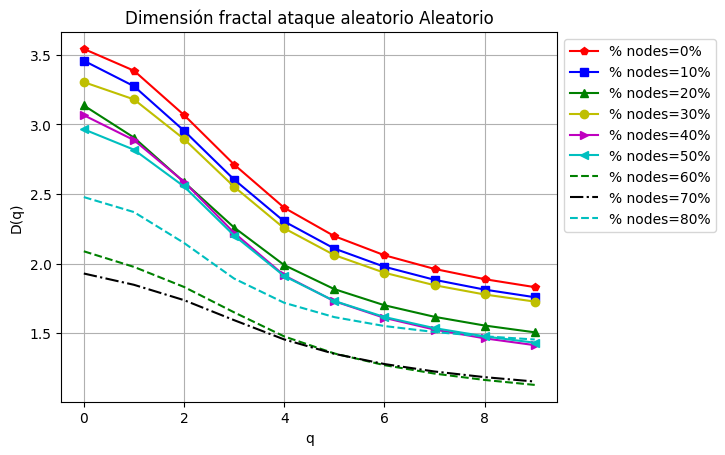
\includegraphics[scale=0.7]{Capitulo6MultifractalidadYRobustez/imagenes/grafica_DqRandom20180512_143117ScaleFree8000Nodes.png}
    \caption{Análisis de multifractalidad de red libre de escala a ataque aleatorio }
\end{figure}

\begin{figure}[H]
    \centering
    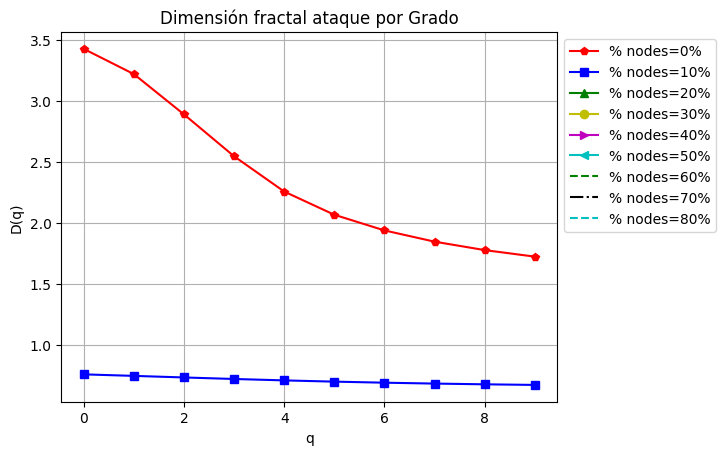
\includegraphics[scale=0.7]{Capitulo6MultifractalidadYRobustez/imagenes/grafica_DqDegree20180512_143117ScaleFree8000Nodes.png}
    \caption{Análisis de multifractalidad de red libre de escala a ataque por grado }
    \label{fig:multfractascalefree}
\end{figure}

\begin{figure}[H]
    \centering
    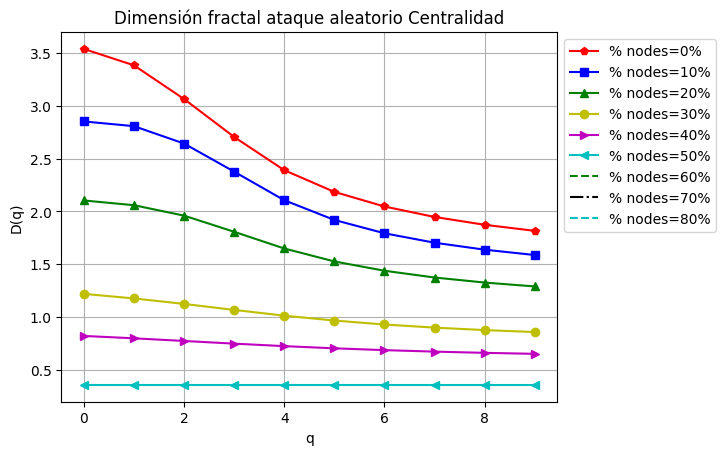
\includegraphics[scale=0.7]{Capitulo6MultifractalidadYRobustez/imagenes/grafica_DqCentrality20180512_143117ScaleFree8000Nodes.png}
    \caption{Análisis de multifractalidad de red libre de escala a ataque por centralidad }
\end{figure}


\begin{figure}[H]
    \centering
    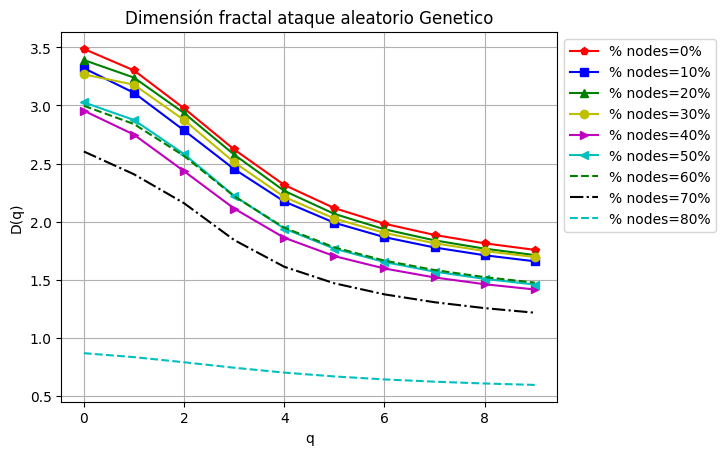
\includegraphics[scale=0.7]{Capitulo6MultifractalidadYRobustez/imagenes/grafica_DqGenetic20180512_143117ScaleFree8000Nodes.png}
    \caption{Análisis de multifractalidad de red libre de escala a ataque por estrategia evolutiva }
\end{figure}

\begin{figure}[H]
    \centering
    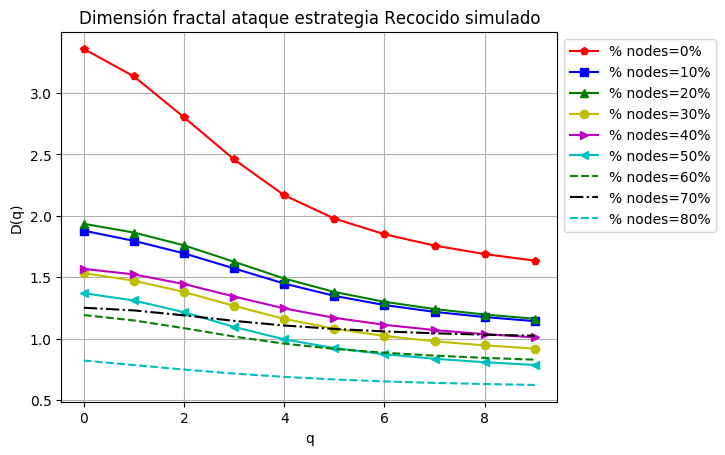
\includegraphics[scale=0.7]{Capitulo6MultifractalidadYRobustez/imagenes/grafica_DqSimulated20180512_143117ScaleFree8000Nodes.png}
    \caption{Análisis de multifractalidad de red libre de escala a ataque por estrategia recocida simulada }
\end{figure}


\subsubsection{Red de mundo pequeño}
\label{sec:multiRobu}
\begin{figure}[H]
    \centering
    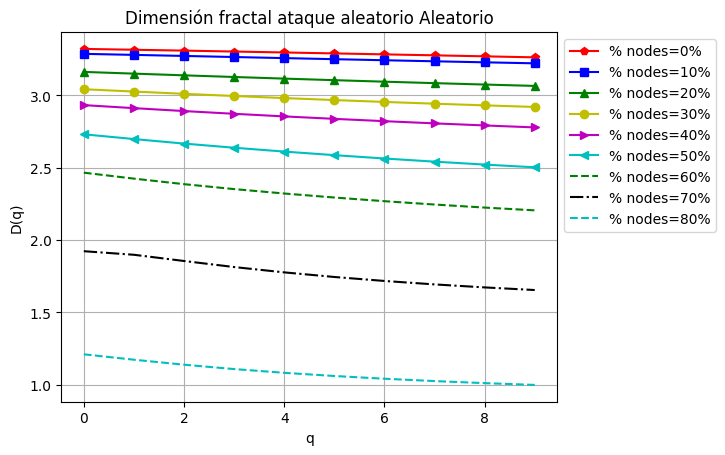
\includegraphics[scale=0.7]{Capitulo6MultifractalidadYRobustez/imagenes/grafica_DqRandom20180510_143549SmallWorld5000NodesRewire01.png}
    \caption{Análisis de multifractalidad de red de mundo pequeño ataque aleatorio }
\end{figure}

\begin{figure}[H]
    \centering
    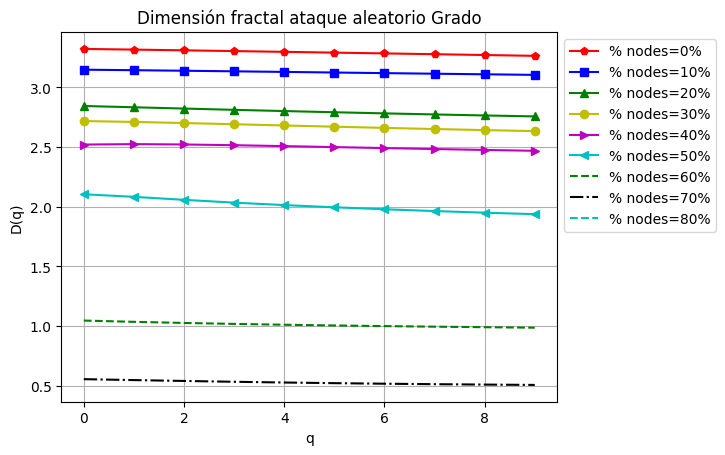
\includegraphics[scale=0.7]{Capitulo6MultifractalidadYRobustez/imagenes/grafica_DqDegree20180510_143549SmallWorld5000NodesRewire01.png}
    \caption{Análisis de multifractalidad de red de mundo pequeño a ataque por grado}
\end{figure}

\begin{figure}[H]
    \centering
    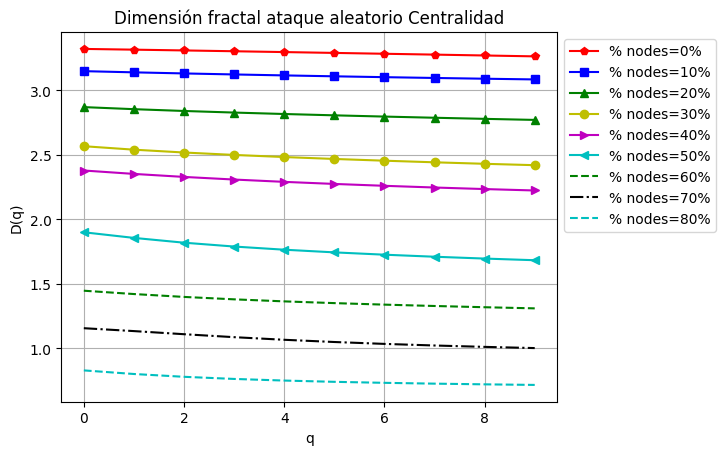
\includegraphics[scale=0.7]{Capitulo6MultifractalidadYRobustez/imagenes/grafica_DqCentrality20180510_143549SmallWorld5000NodesRewire01.png}
    \caption{Análisis de multifractalidad de red de mundo pequeño a ataque por centralidad }
\end{figure}


\begin{figure}[H]
    \centering
    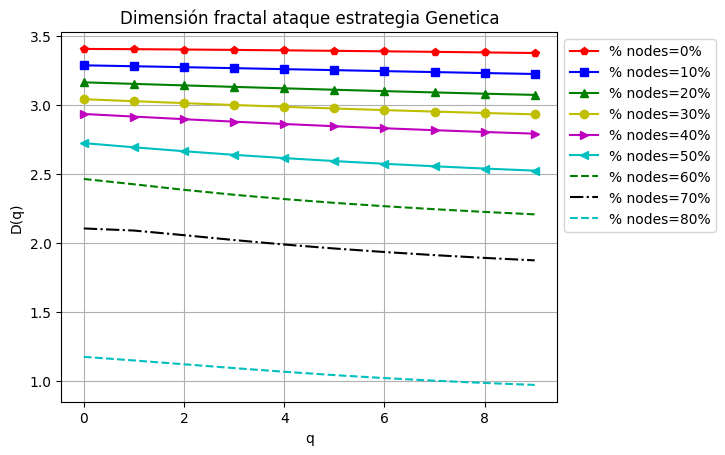
\includegraphics[scale=0.7]{Capitulo6MultifractalidadYRobustez/imagenes/grafica_DqGenetic20180510_143549SmallWorld5000NodesRewire01.png}
    \caption{Análisis de multifractalidad de red red de mundo pequeño a ataque por estrategia evolutiva }
\end{figure}

\begin{figure}[H]
    \centering
    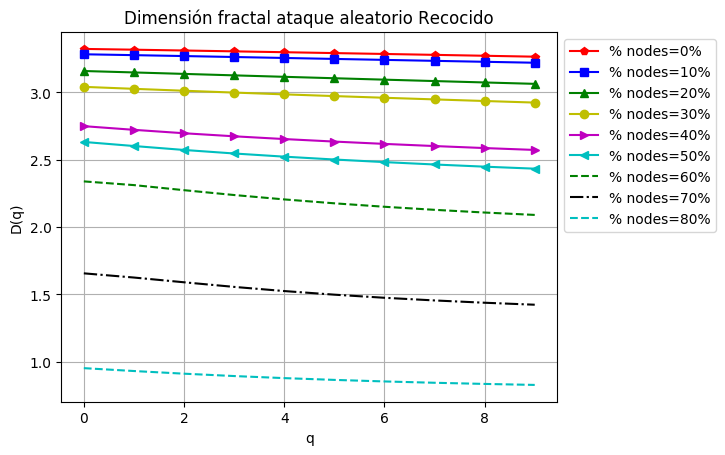
\includegraphics[scale=0.7]{Capitulo6MultifractalidadYRobustez/imagenes/grafica_DqSimulated20180510_143549SmallWorld5000NodesRewire01.png}
    \caption{Análisis de multifractalidad de red de mundo pequeño a ataque por estrategia recocida simulada }
\end{figure}

\subsubsection{Red aleatoria}
\begin{figure}[H]
    \centering
    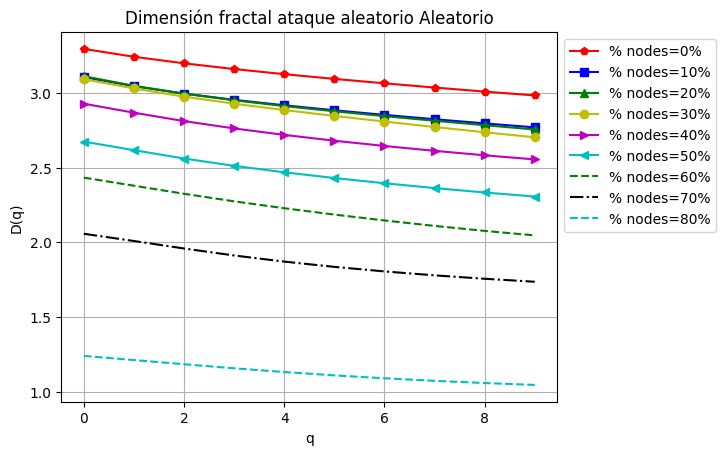
\includegraphics[scale=0.7]{Capitulo6MultifractalidadYRobustez/imagenes/grafica_DqRandom20180501_072543Random1991Nodes5939.png}
    \caption{Análisis de multifractalidad de red aleatoria a ataque aleatorio }
\end{figure}

\begin{figure}[H]
    \centering
    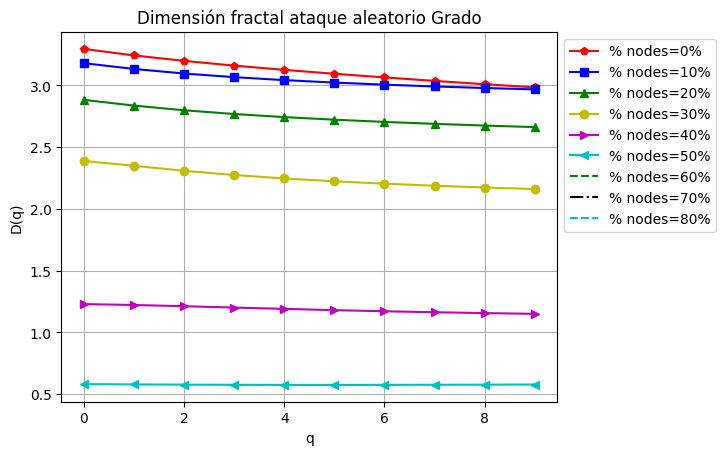
\includegraphics[scale=0.7]{Capitulo6MultifractalidadYRobustez/imagenes/grafica_DqDegree20180501_072543Random1991Nodes5939.png}
    \caption{Análisis de multifractalidad de red aleatoria a ataque por grado }
\end{figure}

\begin{figure}[H]
    \centering
    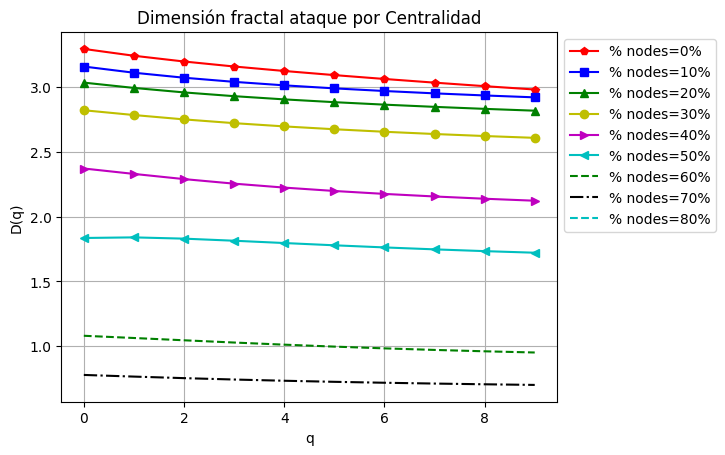
\includegraphics[scale=0.7]{Capitulo6MultifractalidadYRobustez/imagenes/grafica_DqCentrality20180501_072543Random1991Nodes5939.png}
    \caption{Análisis de multifractalidad de red aleatoria a ataque por centralidad}
\end{figure}


\begin{figure}[H]
    \centering
    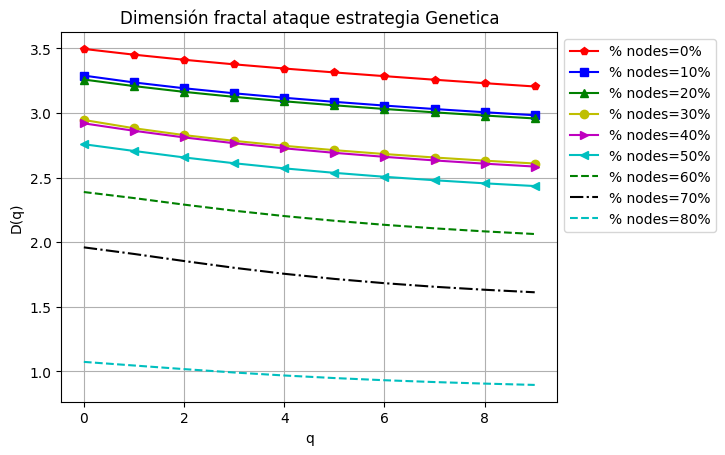
\includegraphics[scale=0.7]{Capitulo6MultifractalidadYRobustez/imagenes/grafica_DqGenetic20180501_072543Random1991Nodes5939.png}
    \caption{Análisis de multifractalidad de red aleatoria a ataque por estrategia evolutiva}
\end{figure}

\begin{figure}[H]
    \centering
    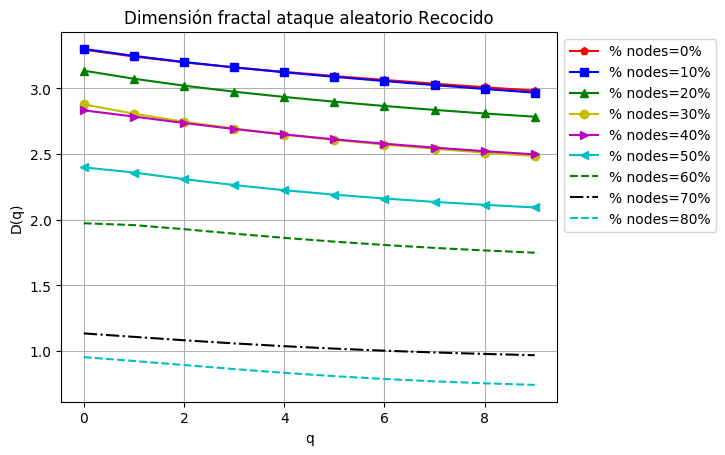
\includegraphics[scale=0.7]{Capitulo6MultifractalidadYRobustez/imagenes/grafica_DqSimulated20180501_072543Random1991Nodes5939.png}
    \caption{Análisis de multifractalidad de red aleatoria a ataque por estrategia recocida simulada }
\end{figure}

\subsubsection{Red real}

\begin{figure}[H]
    \centering
    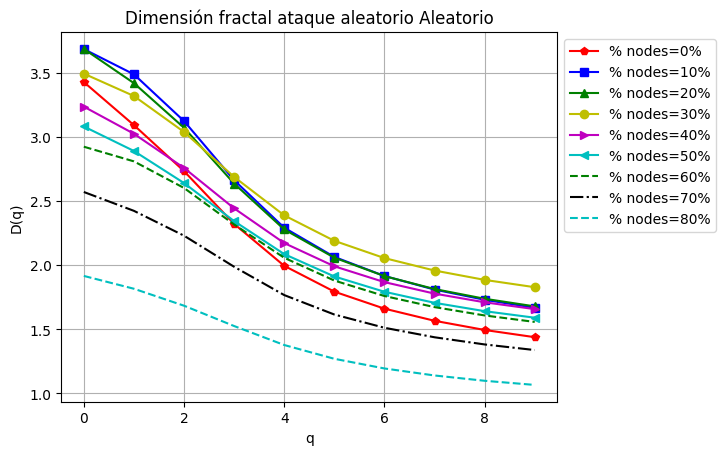
\includegraphics[scale=0.7]{Capitulo6MultifractalidadYRobustez/imagenes/grafica_DqRandom20180508_020345Celengs.png}
    \caption{Análisis de multifractalidad de red observada de Celegens a ataque aleatorio}
\end{figure}

\begin{figure}[H]
    \centering
    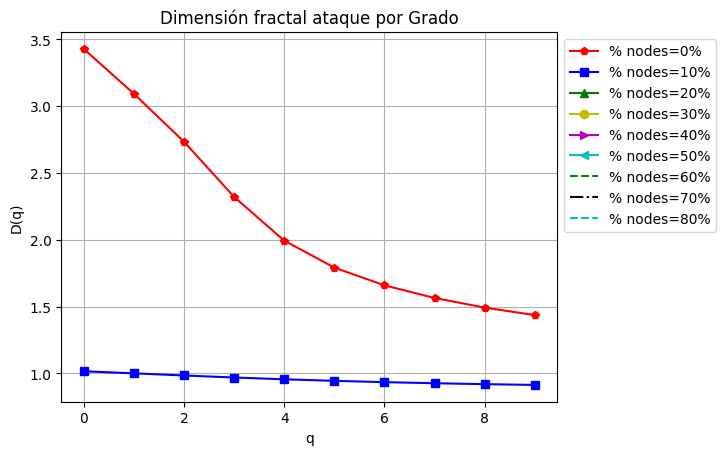
\includegraphics[scale=0.7]{Capitulo6MultifractalidadYRobustez/imagenes/grafica_DqDegree20180508_020345Celengs.png}
    \caption{Análisis de multifractalidad de red observada de Celegens a ataque por grado}
\end{figure}

\begin{figure}[H]
    \centering
    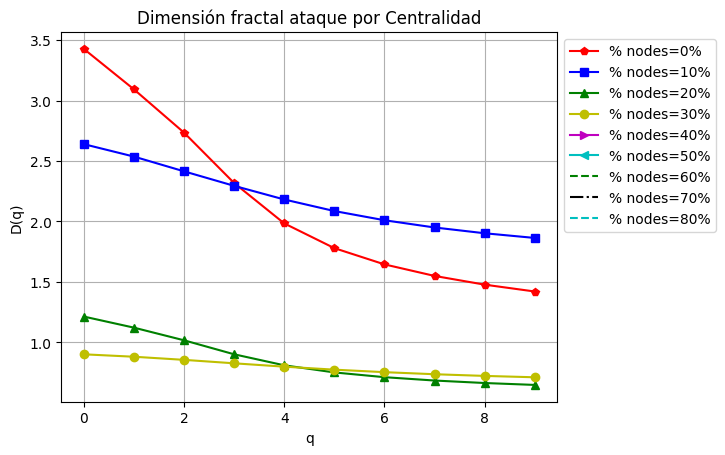
\includegraphics[scale=0.7]{Capitulo6MultifractalidadYRobustez/imagenes/grafica_DqCentrality20180508_020345Celengs.png}
    \caption{Análisis de multifractalidad de red observada de Celegens a ataque por centralidad}
\end{figure}


\begin{figure}[H]
    \centering
    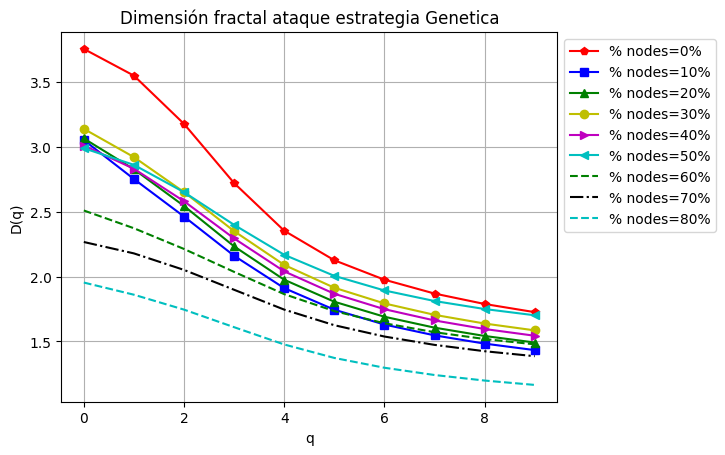
\includegraphics[scale=0.7]{Capitulo6MultifractalidadYRobustez/imagenes/grafica_DqGenetic20180508_020345Celengs.png}
    \caption{Análisis de multifractalidad de red observada de Celegens a ataque por estrategia evolutiva}
\end{figure}

\begin{figure}[H]
    \centering
    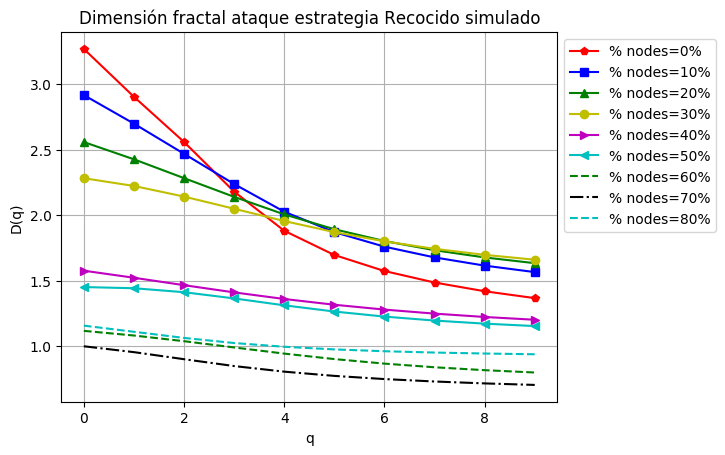
\includegraphics[scale=0.7]{Capitulo6MultifractalidadYRobustez/imagenes/grafica_DqSimulated20180508_020345Celengs.png}
    \caption{Análisis de multifractalidad de red observada de Celegens a ataque por estrategia recocida simulada }
\end{figure}

\subsubsection{Red fractal}
\begin{figure}[H]
    \centering
    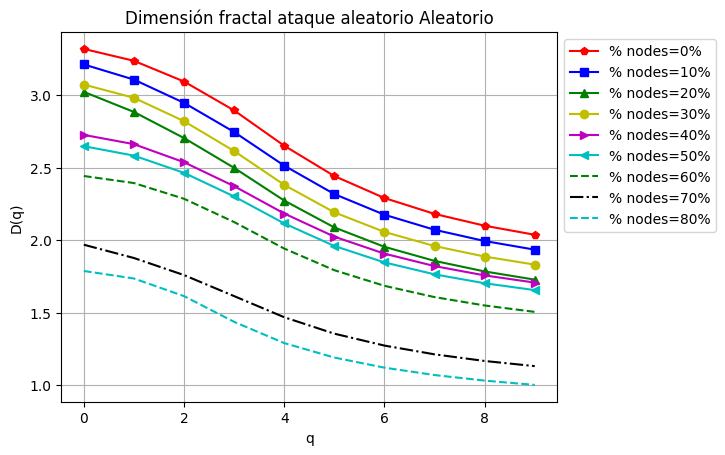
\includegraphics[scale=0.7]{Capitulo6MultifractalidadYRobustez/imagenes/grafica_DqRandom20180501_151350floweru1v3.png}
    \caption{Análisis de multifractalidad de red (1,3)-flower a ataque aleatorio }
\end{figure}

\begin{figure}[H]
    \centering
    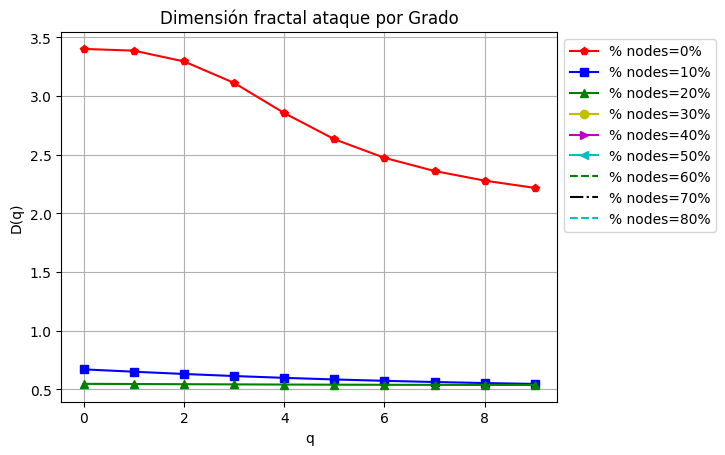
\includegraphics[scale=0.7]{Capitulo6MultifractalidadYRobustez/imagenes/grafica_DqDegree20180501_151350floweru1v3.png}
    \caption{Análisis de multifractalidad de red (1,3)-flower a ataque por grado }
\end{figure}

\begin{figure}[H]
    \centering
    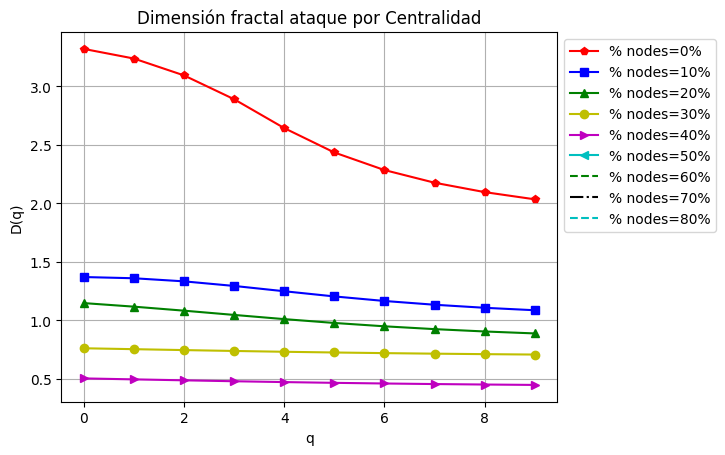
\includegraphics[scale=0.7]{Capitulo6MultifractalidadYRobustez/imagenes/grafica_DqCentrality20180501_151350floweru1v3.png}
    \caption{Análisis de multifractalidad de red (1,3)-flower a ataque por centralidad }
\end{figure}


\begin{figure}[H]
    \centering
    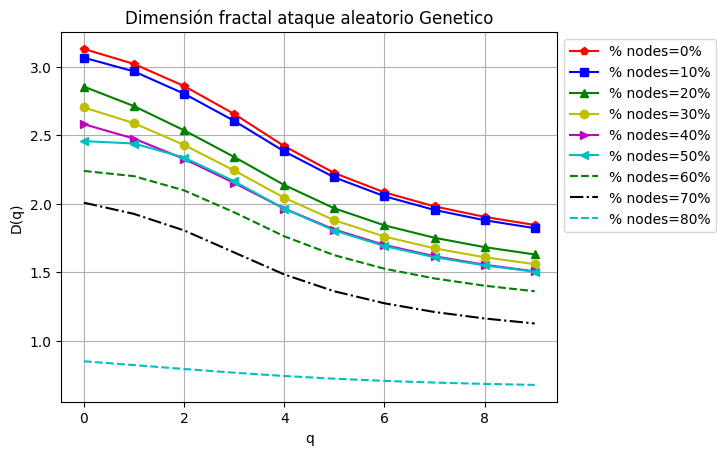
\includegraphics[scale=0.7]{Capitulo6MultifractalidadYRobustez/imagenes/grafica_DqGenetic20180501_151350floweru1v3.png}
    \caption{Análisis de multifractalidad de red (1,3)-flower a ataque por estrategia evolutiva }
\end{figure}

\begin{figure}[H]
    \centering
    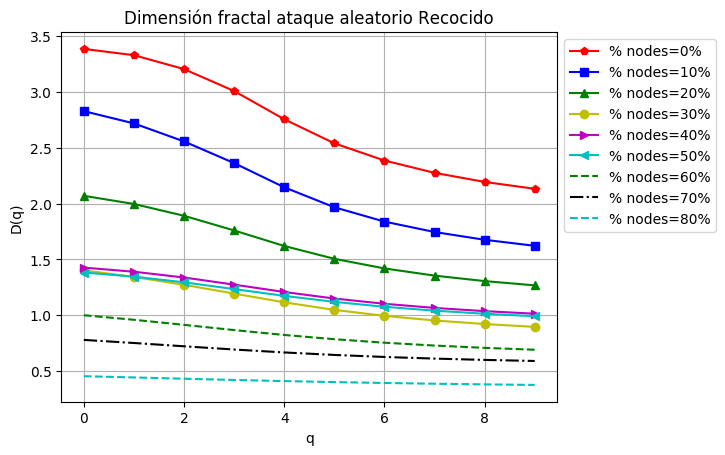
\includegraphics[scale=0.7]{Capitulo6MultifractalidadYRobustez/imagenes/grafica_DqSimulated20180501_151350floweru1v3.png}
    \caption{Análisis de multifractalidad de red (1,3)-flower a ataque por estrategia recocida simulada }
\end{figure}

\subsection{Discusión de resultados}

La relación entre multifractalidad y robustez está dada en como se comporta la dimensión fractal de la red a medida que pierde nodos. Se encuentra que entre más elevada sea la dimensión fractal la red es más robustez, esto se evidencia al cruzar la información, por ejemplo entre la variación del componente gigante \ref{figure:smallWorldGC} y de camino más cortos \ref{figure:smallWorldAPL} sin importar la estrategia de ataque con respecto a la dimensión fractal estudiadas en la sección \ref{sec:multiRobu}.

Así mismo, se encuentra que realizar el análisis de multifractalidad y robustez permite concluir que redes que presentan un gran número de componentes son las más que se adaptan ante fallas aleatorias, ya que las curvas de dimensión fractal presentan poca variación si se pierde un porcentaje pequeño de nodos (10\% o 20\%). En el caso de las redes que tienden a ser monofractales, son las que mejor se adaptan ante cualquier tipo de ataque, ya que el análisis multifractal permite intuir que su estructura interna es compacta, es decir toleran fallos de cualquier tipo.

La estrategia que más efectos produce son las de ataque por grado y centralidad, ya que estas tienden a desintegrar la red. El efecto es tan fuerte, que eliminados un 20\% a 30\% de los nodos, no es posible aplicar los algoritmos de análisis multifractal en algunas redes complejas, ello se evidencia, por ejemplo, en la figura \ref{fig:multfractascalefree}.

Las estrategias de ataque por algoritmos de Inteligencia Artificial, no tienen un efecto tan evidente como lo tienen la centralidad o el grado. Sin embargo, muestran mayor efecto en la redes que las estrategia aleatoria.

Con respecto a las redes de mundo pequeño, se observa que estas conservan su estructura a medida que pierde nodos, lo que muestra que su estructura interna permanece intacta ante diferentes estrategias de ataque.

Para las redes aleatorias, libres de escala, observadas y fractales, se encuentra que pierden su estructura a medida que pierden nodos, pasando de ser objetos multifractales a monofractales. Esto se debe a que estas presentan en mayor o menor medida hubs, los cuales estructuralmente son los centros de estructuras internas, que a medida que se pierden la red se va tornando más uniforme.

En todos los casos, la dimensión fractal tiende hacia 0 a medida que la red pierde nodos, lo que indica que el diámetro de las estructuras internas de la red tiende a cero.